\documentclass[twocolumn]{article}
\usepackage{amsmath}
\usepackage{amsfonts}
\usepackage{amsthm}
\usepackage{graphicx}
\usepackage{thmtools}
\usepackage{hyperref}
\input{sym}

\title{Midterm 1  Review}
\author{Vikas  Dhiman}
\newtheorem{thm}{Theorem}
\newtheorem{defn}{Definition}
\newtheorem{example}{Example}
\newtheorem{prob}{Problem}
\newif\ifsol
\solfalse

\DeclareMathOperator{\atantwo}{arctan2}
\DeclareMathOperator{\tr}{tr}

\begin{document}
\maketitle

\tableofcontents
\section{Linear algebra   review}
\begin{defn}[Matrix] A  real  matrix  $A$ with $n$ rows  and  $m$  columns is defined as a  set  of real numbers  $\{a_{11}, a_{12},
\dots,     a_{nm}\}$, arranged in
an 2D grid with $n$  rows  and $m$  columns :
\begin{align}
  A  =  \begin{bmatrix}
    a_{11}  &  a_{12} &   \dots &  a_{1m} \\
    a_{21}  &  a_{22} &   \dots &  a_{2m} \\
    \vdots  & \vdots &   \ddots  &  \vdots   \\
    a_{n1}  &  a_{n2} &   \dots &  a_{nm} \\
    \end{bmatrix}
\end{align}
\end{defn}

The set of all possible real  matrices with  $n$ rows   and   $m$  columns  is
denoted  as $\bbR^{n \times   m}$, where  $\bbR$ denotes  the set  of all real numbers.

Any matrix $A$ with with  $n$  rows  and  $m$  columns  is   said  to lie  in
the  set  of $\bbR^{n \times   m}$. $A \in \bbR^{n \times m}$  is  read aloud
as ``$A$  lies  in   the set of all $n$ cross $m$  real matrices''.

\begin{defn}[Vector  or Column vector]
  A column vector or a vector $\bfx$ is a matrix  with only one column.
  \begin{align}
    \bfx  =  \begin{bmatrix}
      x_{1} \\
      x_{2} \\
      \vdots   \\
      x_{n} \\
    \end{bmatrix}
  \end{align}
\end{defn}

The set of all possible real  vectors with  $n$ rows   is
denoted  as $\bbR^{n \times   1}$ or more simply $\bbR^{n}$.

A vector is denoted by bold-font small letter, for example, $\bfx, \bfy, \bfz$.
A  matrix is denoted by capital letters, $A, B, M, P, K$.

A matrix $A  \in \bbR^{n \times  m}$ is often denoted a set $m$ column vectors
of dimension $n   \times  1$,
%
\begin{align}
  A  &=  \begin{bmatrix}
    \bfa_1 &  \bfa_2 &  \dots & \bfa_m
  \end{bmatrix},
 \notag\\
 \text{where   }   \bfa_i &= \begin{bmatrix}
 a_{i1} \\  a_{i2} \\ \vdots \\ a_{in}
 \end{bmatrix}, \qquad  \text{ for all } i  \in \{1, \dots, m\}.
\end{align}
%

A block matrix  is a matrix denoted in terms  of  other matrices,
%
\begin{align}
  A &= \left[\begin{array}{ccc|ccc}
        b_{11} & \dots  &   b_{1q}  &   c_{11}  &   \dots   & c_{1r} \\
        \vdots  &  \ddots   & \vdots &  \vdots  &  \ddots  &  \vdots  \\
        b_{p1} & \dots  &   b_{pq}  &   c_{1s}  &   \dots   & c_{sr} \\
        \cline{1-6}  \\
        e_{11} & \dots  &   e_{1v}  &   d_{11}  &   \dots   & d_{1x} \\
        \vdots  &  \ddots   & \vdots &  \vdots  &  \ddots  &  \vdots  \\
        e_{u1} & \dots  &   e_{uv}  &   d_{1w}  &   \dots   & d_{wx} \\
            \end{array}\right]
  \\
    &= \begin{bmatrix}
        B  &   C \\
        E & D
        \end{bmatrix}, \text{  where  }  B, C, E, D \text{ are matrices.}
\end{align}
%

\begin{defn}[Square matrix]
  A matrix is said to be square if its number of columns is same as the number
  of rows. That is matrix   $A \in \bbR^{n \times m}$ is said to be square
  matrix if $m = n$.
\end{defn}

\begin{defn}[Diagonal of a square matrix]
  Let $A$ be a square matrix $A \in \bbR^{n \times n}$  with   entries:
  \begin{align}
    A  =  \begin{bmatrix}
      a_{11}  &  a_{12} &   \dots &  a_{1n} \\
      a_{21}  &  a_{22} &   \dots &  a_{2n} \\
      \vdots  & \vdots &   \ddots  &  \vdots   \\
      a_{n1}  &  a_{n2} &   \dots &  a_{nn} \\
    \end{bmatrix}
  \end{align}
  The diagonal of a square matrix  $A$ is defined  to be the vector
  \[  \text{diag}(A)= \begin{bmatrix} a_{11} \\   a_{22} \\ \vdots  \\ a_{nn} \end{bmatrix}\]
\end{defn}


\begin{defn}[Trace of a square matrix]
  Trace  of a square matrix  $A$ is defined as the sum its diagonal elements,
  \[ \tr(A) = \sum_{i=1}^n a_{ii} \].
\end{defn}

\begin{defn}[Identity matrix]
  An identity matrix $I$ of size $n$ is  a square matrix with all its diagonal
  entries as 1 and non-diagonal entries as 0.
  \begin{align}
    I  =  \begin{bmatrix}
      1 & 0 & \dots & 0   \\
      0 & 1 & \dots & 0   \\
      \vdots   & \vdots &  \ddots  & \vdots \\
      0 & 0 & \dots & 1   \\
      \end{bmatrix}
    \end{align}
\end{defn}


\subsection{Matrix operations}
\subsubsection{Transpose}
\begin{defn}[Transpose]
  The matrix transpose $A^\top$ of a matrix $A$ is defined as a matrix where
  rows of matrix $A$ are the columns  of $A^\top$ and vice-versa.
  \begin{align}
    A^\top  =  \begin{bmatrix}
      a_{11}  &  a_{21} &   \dots &  a_{1n} \\
      a_{12}  &  a_{22} &   \dots &  a_{2n} \\
      \vdots  & \vdots &   \ddots  &  \vdots   \\
      a_{1m}  &  a_{2m} &   \dots &  a_{nm} \\
    \end{bmatrix}
  \end{align}
\end{defn}

In  the matrix as set of  $m$ column  vectors notation, the transpose is written as $m$
row  vectors $\bfa_i^\top$,
%
\begin{align}
  A^\top  &=  \begin{bmatrix}
    \bfa_1^\top \\ \bfa_2^\top \\ \vdots \\  \bfa_m^\top
  \end{bmatrix},
  \quad
  \bfa_i^\top = \begin{bmatrix}
    a_{i1}  & a_{i2}  &   \dots &  a_{in}
  \end{bmatrix},
                                  \notag \\
  &\qquad \text{for all } i \in \{1, \dots, n\}.
\end{align}
%

\begin{enumerate}
\item  If $A$ has $n$rows and  $m$  columns, then  $A^\top$  has $m$ rows and
  $n$  columns. If  $A \in \bbR^{n \times  m}$, then  $A^\top \in \bbR^{m
    \times n}$.
  \item  The transpose  of  a transpose is matrix itself. $(A^\top)^\top = A$.
  \item  The transpose of a block matrix is  block-wise  transpose  of  each
    matrix,
    \[
    \begin{bmatrix}
      B  &   C \\
      E & D
    \end{bmatrix}^\top
    = 
    \begin{bmatrix}
      B^\top  & E^\top \\
      C^\top & D^\top
    \end{bmatrix}
    \]
    
\end{enumerate}


\begin{defn}[Row vector]
  A row vector is $Y$ is matrix  with only one row
  \begin{align}
    Y  =  \begin{bmatrix}
      y_{1} &
      y_{2} &
      \dots  &
      y_{n}
    \end{bmatrix}
  \end{align}
\end{defn}
It is common  to denote row vectors as tranpose  of  a  column vector. For
example, the  matrix  $Y$ shown above is typically represented  $\bfy^\top$, where
$\bfy$  is a column vector.
%
  \begin{align}
    Y  &=  \bfy^\top & \text{ where } \bfy = \begin{bmatrix}
      y_{1} \\
      y_{2} \\
      \vdots  \\
      y_{n}
    \end{bmatrix}
  \end{align}

\subsubsection{Vector dot product}
Before we define  general matrix multiplication, it  is easier to define matrix
multiplication   between a row vector and a column vector $\bfx^\top  \in
\bbR^{1 \times  n}$ and $\bfy\in\bbR^{n \times 1}$
%
\begin{align}
  \bfx^\top \bfy  &= x_1y_1 + x_2 y_2 + \dots  + x_n y_n = \sum_{i=1}^n  x_iy_i
\\
\text{where }  \bfx^\top &=  \begin{bmatrix} x_1 &  \dots  &  x_n \end{bmatrix}
\notag \\
  \text{  and  }\bfy &=  \begin{bmatrix} y_1 \\  \vdots  \\  y_n \end{bmatrix}.
  \notag
\end{align}
%
Note that $\bfx^\top \bfy$   is same as the vector  dot product  or the vector
inner-product,
%
\begin{align}
  \bfx^\top \bfy = \bfx \cdot \bfy  =  \|\bfx\|\|\bfy\|cos(\theta) = \bfy^\top \bfx,
\end{align}
  %
where  $\theta$  is the angle between   vectors $\bfx$ and $\bfy$ and  the
vector norm  or euclidean norm $\|.\|$ is defined as
%
\begin{align}
  \|\bfx\| =  \sqrt{x_1^2 + x_2^2  +   \dots +  x_n^2} = \sqrt{\bfx^\top\bfx}
\end{align}
%

\begin{defn}[Unit  vector]
  A unit vector, typically denoted  with a hat, $\hat{\bfx}$ is a vector with
  euclidean norm as 1. That is  $\|\hat{\bfx}\| = 1$ or equivalently
  $\bfx^\top\bfx =  1$.
\end{defn}

\begin{defn}[Orthogonal vectors]
  Two vectors, $\bfx \in  \bbR^n$  and $\bfy \in \bbR^n$ are said to be
  orthogonal if and only if their dot product is zero $\bfx^\top \bfy =  0$.
\end{defn}

\begin{defn}[Orthonormal vectors]
  A set of vectors, $\bfx_1, \bfx_2, \dots, \bfx_n \in  \bbR^n$  are said to be
  orthonormal if and only if they are all  unit vectors $\bfx_i^\top\bfx_i  = 1$
  and they are  pair-wise orthogonal, $\bfx_i^\top  \bfx_j =  0$ for all $i \ne j$. 
\end{defn}

\subsubsection{Matrix multiplication}
The matrix multiplication between  matrix  $A \in \bbR^{n  \times m}$   and
matrix $B  \in \bbR^{m \times p}$ (note that $A$ has $m$ columns while B has $m$
rows;  the only case when matrix multiplication  is defined) is easier 
defined if matrix $A$  is written in terms  of row vectors while  matrix  $B$ is
written  in  terms  of column vectors. Let  the  matrix $A$  is written in terms
of row   vectors $\bfa_i^\top   \in \bbR^{1 \times m}$ and the matrix $B$ is written in terms of column
vectors $\bfb_i \in \bbR^{m \times  1}$. Then the matrix multiplication $AB \in
\bbR^{n \times  p}$ is defined as the matrix,
%
\begin{align}
  AB &= \begin{bmatrix}
    \bfa_1^\top
    \\
    \bfa_2^\top
    \\
    \vdots
    \\
    \bfa_n^\top
    \end{bmatrix}
  \begin{bmatrix}
    \bfb_1
    &
    \bfb_2
    &
    \dots
    &
    \bfb_p
  \end{bmatrix}
      \\
  &= \begin{bmatrix}
    \bfa_1^\top\bfb_1 & \bfa_1^\top\bfb_2 &  \dots & \bfa_n^\top \bfb_p
    \\
    \bfa_2^\top\bfb_1 & \bfa_2^\top\bfb_2 &  \dots & \bfa_n^\top \bfb_p
    \\
    \vdots &  \vdots  &  \ddots  &   \vdots
    \\
    \bfa_n^\top\bfb_1 & \bfa_n^\top\bfb_2 &  \dots & \bfa_n^\top \bfb_p
    \end{bmatrix}
\end{align}

\paragraph{Block matrix  multiplication}
Block matrix multiplication works in a similar way  as scalar multiplication as
long as sub-matrix multiplication is properly defined,
%
\begin{align}
  \begin{bmatrix}  A & B \\  C &  D \end{bmatrix}
  \begin{bmatrix}  P & Q \\  R &  S \end{bmatrix}
 =
   \begin{bmatrix}  AP+BR & AQ+BS \\  CP+DR &  CQ+DS \end{bmatrix}
  \end{align}
  %

\begin{defn}[Orthogonal matrices]
  A square matrix $A$ is said to be orthogonal if and only if $A^\top A = I$
\end{defn}

\subsubsection{Transpose of matrix multiplication}
\[
  (AB)^\top = B^\top A^\top
  \]

\subsubsection{Properties of trace  operator}
Trace is a linear operator:
\begin{align}
  \tr(\alpha A  +  \beta B) = \alpha \tr(A) +  \beta \tr(B),
\end{align}
for compatible matrices  $A$ and $B$   and scalars $\alpha$ and $\beta$.

\section{Gaussian elimination or  $LDU$  factorization}
A system  of  equations   $A\bfx =  \bfb$  can  be  solved by  Gaussian
elimination or   equivalently factorizing   $A$  into  triangular
factorization    also   known  as   $LDU$  factorization. After  this
factorization, the  matrix $A \in  \bbR^{n \times n}$ is factorized into
lower-triangular matrix $L$, diagonal matrix $D$ and  uppper-triangular   matrix
$U$. Sometimes a permutation matrix $P$  is  also required. The  factorization
is  such  that   $PA = LDU$.
Let  us   write  the  matrix   $A$ in   terms   of   its    elements  $a_{ij}$.
Also let  us   denote the $i$th    row of matrix $A$  as $\bfr_i^\top   =   [a_{i1},
\dots,   a_{in}]$.
\begin{align}
  A   =  \begin{bmatrix}
    a_{11} & a_{12}  &   \dots &  a_{1n} \\
    a_{21} & a_{22}  &   \dots &  a_{2n} \\
    \vdots &  \vdots  & \ddots & \vdots \\
    a_{n1} & a_{n2}  &   \dots &  a_{nn}
    \end{bmatrix}  =  \begin{bmatrix}  \bfr_1^\top  \\  \bfr_2^\top \\ \vdots \\ \bfr_n^\top\end{bmatrix}.
\end{align}
To consider  the  simplest  case, we   assume that $a_{11}
\ne 0$.  If  this is not the case, rearrange the rows of $A$ such that $a_{11}
\ne 0$. We want  to make the first element of  the second row to  be zero. This  can  be achieved if  we subtract $\bfr'^\top_2 =  \bfr_2^\top -
\frac{a_{21}}{a_{11}}   \bfr_1^\top$, where $\bfr'^\top_2$ is  the  new  row
after the  operation. This is  equivalent to multiplying both sides
by a  matrix:
\begin{align*}
 &\begin{bmatrix} 1  & 0  &  0 &  \dots  & 0 \\
  -\frac{a_{21}}{a_{11}} & 1  & \dots  &   0  \\
  0 & 0  & 1 & \dots  &   0  \\
  \vdots  & \vdots &  \vdots  &   \ddots  &  \vdots   \\
  0 & 0 &  0   &  \dots  & 1
\end{bmatrix}A  \\
&=  \scalebox{0.8}{\mbox{$\begin{bmatrix}
  a_{11} & a_{12}  &  a_{13} &     \dots &  a_{1n} \\
  0 & a_{22}-\frac{a_{21}}{a_{11}}a_{12}  & a_{23}-\frac{a_{21}}{a_{11}}a_{13} &  \dots &  a_{2n} -\frac{a_{21}}{a_{11}}a_{1n}\\
  a_{31} & a_{32}  &  a_{33} &     \dots &  a_{3n} \\
  \vdots &  \vdots  & \vdots &  \ddots & \vdots \\
  a_{n1} & a_{n2}  &  a_{n3} &   \dots &  a_{nn}
\end{bmatrix}$}}.
\end{align*}
This makes  sure   that  the  first element  of   second   row is zero.  Since
we  want  the    represent   matrix $A$   as a    factorization, we want to
represent the  matrix  operation as one   that   restores  the  ``un-does'' the
operation   $\bfr_2^{'\top}=\bfr_2^\top - \frac{a_{21}}{a_{11}}\bfr_1^\top$, to
get back  the  matrix $A$. Such
an  operation is  $\bfr_2^\top  =\bfr_2^{'\top}+
\frac{a_{21}}{a_{11}}\bfr_1^\top$.  So we  can  re-write the matrix  $A$ as,
%
\begin{align*}
  &A=\begin{bmatrix} 1  & 0  &  0 &  \dots  & 0 \\
    \frac{a_{21}}{a_{11}} & 1  & \dots  &   0  \\
    0 & 0  & 1 & \dots  &   0  \\
    \vdots  & \vdots &  \vdots  &   \ddots  &  \vdots   \\
    0 & 0 &  0   &  \dots  & 1
  \end{bmatrix}  \\
  &  \scalebox{0.8}{\mbox{$\begin{bmatrix}
        a_{11} & a_{12}  &  a_{13} &     \dots &  a_{1n} \\
        0 & a_{22}-\frac{a_{21}}{a_{11}}a_{12}  & a_{23}-\frac{a_{21}}{a_{11}}a_{13} &  \dots &  a_{2n} -\frac{a_{21}}{a_{11}}a_{1n}\\
        a_{31} & a_{32}  &  a_{33} &     \dots &  a_{3n} \\
        \vdots &  \vdots  & \vdots &  \ddots & \vdots \\
        a_{n1} & a_{n2}  &  a_{n3} &   \dots &  a_{nn}
      \end{bmatrix}$}}.
\end{align*}
%
A  similar  operation  can  be applied to  all rows for  $i \ge 2$ to make  their first element
to  be zero, $\bfr_i^{'\top} =  \bfr_i^\top  -\frac{a_{i1}}{a_{11}} \bfr_1^\top$
for all $i \ge 2$.
% 
\begin{align*}
  &A=\begin{bmatrix} 1  & 0  &  0 &  \dots  & 0 \\
    \frac{a_{21}}{a_{11}} & 1  & \dots  &   0  \\
    \frac{a_{31}}{a_{11}} & 0  & 1 & \dots  &   0  \\
    \vdots  & \vdots &  \vdots  &   \ddots  &  \vdots   \\
    \frac{a_{n1}}{a_{11}} & 0 &  0   &  \dots  & 1
  \end{bmatrix}  \\
  &  \scalebox{0.8}{\mbox{$\begin{bmatrix}
        a_{11} & a_{12}  &  a_{13} &     \dots &  a_{1n} \\
        0 & a_{22}-\frac{a_{21}}{a_{11}}a_{12}  & a_{23}-\frac{a_{21}}{a_{11}}a_{13} &  \dots &  a_{2n} -\frac{a_{21}}{a_{11}}a_{1n}\\
        0 & a_{32} -\frac{a_{31}}{a_{11}}a_{13} &  a_{33}-\frac{a_{31}}{a_{11}}a_{13} &     \dots &  a_{3n}-\frac{a_{31}}{a_{11}}a_{1n} \\
        \vdots &  \vdots  & \vdots &  \ddots & \vdots \\
        0 & a_{n2}-\frac{a_{n1}}{a_{11}}a_{12}  &  a_{n3} -\frac{a_{n1}}{a_{11}}a_{13}&   \dots &  a_{nn}-\frac{a_{n1}}{a_{11}}a_{1n}
      \end{bmatrix}$}}.
\end{align*}
% 
Thus we  have made first  column   zero below  the  diagonal  on  the  second
matrix. As long $a'_{22} = a_{22} - \frac{a_{21}}{a_{11}}a_{12} \ne 0$,  a  similar procedure  can be  applied to the make the second
column  zero  below   the  diagonal. If $a'_{22} = 0$, then swap the second row
with a row whos second  element is non-zero. If all  rows  have   second element
as zero then this step  is done,  target  to   make  the third column  below to
be zero.  Denote the  second  column  elements  for
row  $i \ge 2$ by
$a'_{ij} = a_{ij}  - \frac{a_{i1}}{a_{11}}a_{1j}$.  Then   the  operation
$\bfr_{i}^{''\top} = \bfr_i^{'\top}  - \frac{a'_{i2}}{a'_{22}}\bfr_2^{'\top}$  for all
$i \ge 3$, will
make the second  column below diagonal  to be  zero. And the matrix
factorization will look  like,
% 
\begin{align*}
  &A=\begin{bmatrix} 1  & 0  &  0 &  \dots  & 0 \\
    \frac{a_{21}}{a_{11}} & 1  & \dots  &   0  \\
    \frac{a_{31}}{a_{11}} & \frac{a'_{32}}{a'_{22}}  & 1 & \dots  &   0  \\
    \vdots  & \vdots &  \vdots  &   \ddots  &  \vdots   \\
    \frac{a_{n1}}{a_{11}} & \frac{a'_{n2}}{a'_{22}} &  0   &  \dots  & 1
  \end{bmatrix}  \\
  &  \scalebox{0.8}{\mbox{$\begin{bmatrix}
        a_{11} & a_{12}  &  a_{13} &     \dots &  a_{1n} \\
        0 & a_{22}-\frac{a_{21}}{a_{11}}a_{12}  & a_{23}-\frac{a_{21}}{a_{11}}a_{13} &  \dots &  a_{2n} -\frac{a_{21}}{a_{11}}a_{1n}\\
        0 & 0 &  a'_{33}-\frac{a'_{32}}{a'_{22}}a'_{23} &     \dots &  a'_{3n}-\frac{a'_{32}}{a'_{22}}a'_{2n} \\
        \vdots &  \vdots  & \vdots &  \ddots & \vdots \\
        0 & 0  &  a_{n3} -\frac{a'_{n1}}{a'_{22}}a'_{23}&   \dots &  a'_{nn}-\frac{a'_{n2}}{a'_{22}}a'_{2n}
      \end{bmatrix}$}}.
\end{align*}
% 
One can  continue this  procedure  until  the second matrix  is all  0's  below
the  diagonal (upper-triangular)   while  maintaining  that  the  first matrix
is  all  0's above the  diagonal, (lower-triangular),
% 
\begin{align*}
  &A=\begin{bmatrix} 1  & 0  &  0 &  \dots  & 0 \\
    \frac{a_{21}}{a_{11}} & 1  & \dots  &   0  \\
    \frac{a_{31}}{a_{11}} & \frac{a'_{32}}{a'_{22}}  & 1 & \dots  &   0  \\
    \vdots  & \vdots &  \vdots  &   \ddots  &  \vdots   \\
    \frac{a_{n1}}{a_{11}} & \frac{a'_{n2}}{a'_{22}} &  \frac{a''_{n3}}{a''_{n3}}   &  \dots  & 1
  \end{bmatrix}  \\
  &  \scalebox{0.8}{\mbox{$\begin{bmatrix}
        a_{11} & a_{12}  &  a_{13} &     \dots &  a_{1n} \\
        0 & a_{22}-\frac{a_{21}}{a_{11}}a_{12}  & a_{23}-\frac{a_{21}}{a_{11}}a_{13} &  \dots &  a_{2n} -\frac{a_{21}}{a_{11}}a_{1n}\\
        0 & 0 &  a'_{33}-\frac{a'_{32}}{a'_{22}}a'_{23} &     \dots &  a'_{3n}-\frac{a'_{32}}{a'_{22}}a'_{2n} \\
        \vdots &  \vdots  & \vdots &  \ddots & \vdots \\
        0 & 0  &  0&   \dots &  u_{nn}
      \end{bmatrix}$}}.
\end{align*}
% 
The  first  matrix is denoted   as  $L$   while the   second matrix  is  denoted
as $DU$.  The second  matrix    can  be   factorized into   diagonal matrix  $D$
and
upper-triangular matrix  $U$ so that $U$ matrix has diagonal elements as $1$,

\begin{align*}
  &A=LDU\\
  &\text{ where   } L =  \begin{bmatrix} 1  & 0  &  0 &  \dots  & 0 \\
    \frac{a_{21}}{a_{11}} & 1  & \dots  &   0  \\
    \frac{a_{31}}{a_{11}} & \frac{a'_{32}}{a'_{22}}  & 1 & \dots  &   0  \\
    \vdots  & \vdots &  \vdots  &   \ddots  &  \vdots   \\
    \frac{a_{n1}}{a_{11}} & \frac{a'_{n2}}{a'_{22}} &  \frac{a''_{n3}}{a''_{n3}}   &  \dots  & 1
  \end{bmatrix}\\
  &DU = \scalebox{0.8}{\mbox{$\begin{bmatrix}
        a_{11} & a_{12}  &  a_{13} &     \dots &  a_{1n} \\
        0 & a_{22}-\frac{a_{21}}{a_{11}}a_{12}  & a_{23}-\frac{a_{21}}{a_{11}}a_{13} &  \dots &  a_{2n} -\frac{a_{21}}{a_{11}}a_{1n}\\
        0 & 0 &  a'_{33}-\frac{a'_{32}}{a'_{22}}a'_{23} &     \dots &  a'_{3n}-\frac{a'_{32}}{a'_{22}}a'_{2n} \\
        \vdots &  \vdots  & \vdots &  \ddots & \vdots \\
        0 & 0  &  0&   \dots &  u'_{nn}
      \end{bmatrix}$}}
\end{align*}
% 
Let the elements of upper-triangular $DU$ matrix  be denoted  by $u'_{ij}$,
%
\begin{align*}
  DU &= \begin{bmatrix}
    u'_{11} & u'_{12}  &   \dots &  u'_{1n} \\
    0 & u'_{22}  &   \dots &  u'_{2n} \\
    \vdots &  \vdots  & \ddots & \vdots \\
    0 & 0  &   \dots &  u'_{nn}
      \end{bmatrix}.
\end{align*}
%
Such  a matrix  can be factorized into diagonal  matrix  $D$  and $U$
where $D$ has the diagonal elements of $U$ while  $U$  rows  are  divided  by
the  diagonal element,
%
\begin{align*}
  D &= \begin{bmatrix}
    u'_{11} & 0  & 0  &  \dots &  0 \\
    0 & u'_{22}  & 0   &   \dots &  0 \\
    0 & 0   & u'_{33}  &   \dots &  0 \\
    \vdots &  \vdots  & \vdots  & \ddots & \vdots \\
    0 & 0  &   0   & \dots &  u'_{nn}
  \end{bmatrix}.
                       \\
  U  &=  \begin{bmatrix}
    1 & \frac{u'_{12}}{u'_{11}} & \frac{u'_{13}}{u'_{11}} &   \dots &  \frac{u'_{1n}}{u'_{11}} \\
    0 & 1  &   \frac{u'_{23}}{u'_{22}} &   \dots &  \frac{u'_{2n}}{u'_{22}} \\
    0 & 0  &   1 & \dots &  \frac{u'_{3n}}{u'_{33}} \\
    \vdots &  \vdots  & \vdots  & \ddots & \vdots \\
    0 & 0  &   0 &  \dots &  1
  \end{bmatrix}
\end{align*}

\begin{example}
  Let $A$ be   the  matrix,
  \[
    A   =  \begin{bmatrix}
      1 &   2  &  3  \\
      4 & 5 &   6 \\
      2 & 4 &   6
    \end{bmatrix}
    \]
\begin{enumerate}
  \item  Step  1: Row 2 = Row  2 -  4 times Row  1  or $\bfr_2^{'\top} =
    \bfr_2^\top  -  4 \bfr_1^\top$.
    \[
      A   =  \begin{bmatrix}
        1 &   2  &  3  \\
        4 & 5 &   6 \\
        2 & 4 &   6
      \end{bmatrix}
      =   \begin{bmatrix}
        1 & 0  &  0 \\
        4  &  1 &  0  \\
        0  &  0 &  1
        \end{bmatrix}\begin{bmatrix}
        1 & 2 &  3  \\
        0 & -3 &  -6 \\
        2 & 4 &  6
      \end{bmatrix}
    \]
    The  first  matrix ``un-does'' $\bfr_2^{'\top} =
    \bfr_2^\top  -  4 \bfr_1^\top$, because  it  operates  $\bfr_2^{\top} =
    \bfr_2^{'\top}  +  4 \bfr_1^\top$    on  the   second  matrix  to get back $A$.
  \item Step 2: Row  3  =   Row  3 - 2  times row 1  or   $\bfr_3^{'\top} =
    \bfr_3^\top  -  2 \bfr_1^\top$,
    \[
      A   =  \begin{bmatrix}
        1 &   2  &  3  \\
        4 & 5 &   6 \\
        2 & 4 &   6
      \end{bmatrix}
      =   \begin{bmatrix}
        1 & 0  &  0 \\
        4  &  1 &  0  \\
        2  &  0 &  1
      \end{bmatrix}\begin{bmatrix}
        1 & 2 &  3  \\
        0 & -3 &  -6 \\
        0 & 0 &  0
      \end{bmatrix}
    \]
    We do   not need to do any more  operations because we already got
    lower-triangular  and  upper-triangular   decomposition.  We can separate
    the diagonal from the  upper-triangular  matrix,

    \item  Step   3:  Separate  the diagonal components  from upper-triangular matrix,
    \[
      A   
      =   \underbrace{\begin{bmatrix}
        1 & 0  &  0 \\
        4  &  1 &  0  \\
        2  &  0 &  1
      \end{bmatrix}}_{L}
      \underbrace{\begin{bmatrix}
        1 & 0 &  0  \\
        0 & -3 &  0 \\
        0 & 0 &  0
      \end{bmatrix}}_{D}
      \underbrace{\begin{bmatrix}
        1 & 2 &  3  \\
        0 & 1 &  2 \\
        0 & 0 &  0
      \end{bmatrix}}_{U}
    \]
\end{enumerate}
\end{example}



\section{Trignometry review}
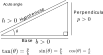
\includegraphics[width=\linewidth]{media/trig.pdf}

\section{Triangle law of vector addition}
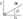
\includegraphics[width=\linewidth]{media/triangle-law.png}

\section{2D  Rotation matrix}
\begin{defn}[2D  Cartesian Coordinate frame]
 A 2D cartesian coordinate  frame  is defined as a set of mutually orthogonal unit
 vectors  $\hat{\bfx} \in  \bbR^2$  and
 $\hat{\bfy}\in  \bbR^2 $ called the basis vectors $B = [\hat{\bfx}, \hat{\bfy}]$
 along  with  an origin  $\bfo\in  \bbR^2$. Thus the tuple  $(B, \bfo)$ form a
 coordinate frame. A  coordinate  frame is denoted  by curly braces around it,
 for  example, $\{C\}$ or $\{W\}$.
\end{defn}

\begin{example}[2D Coordinate frame]
  The figure~\ref{fig:rot-2D} contains two coordinate frames the one  shown  in
  red and   the one   shown in green. Both have  the  same origin, but
  different  basis vectors. The $\{W\}$ coordinate frame shown in green has
  basis vectors $B_w = [\hat{\bfx}_w, \hat{\bfy}_w]$. The same notation is used
  for the $\{C\}$ coordinate frame $B_c  =  [ \hat{\bfx}_c, \hat{\bfy}_c]$.
  Note that the basis vectors of $\{C\}$  coordinate frame  can be
  expressed  in  terms of $\{W\}$  coordinate frame by triangle  law of vector addition,
  \begin{equation}
  \begin{aligned}
    \hat{\bfx}_c &= |\overrightarrow{OA}|\hat{\bfx}_w + |\overrightarrow{AB}|\hat{\bfy}_w
    \\
    \hat{\bfy}_c &= -|\overrightarrow{PQ}|\hat{\bfx}_w + |\overrightarrow{OP}|\hat{\bfy}_w
  \end{aligned}
  \label{eq:c-as-w}
  \end{equation}

  In the  triangle $\Delta OAB$ (Fig~\ref{fig:rot-2D}),
  \begin{align}
    \cos(\theta) &= \frac{|\overrightarrow{OA}|}{|\overrightarrow{OB}|}
                   = \frac{|\overrightarrow{OA}|}{\|\hat{\bfx}_c\|} = |\overrightarrow{OA}| \\
    \sin(\theta) &= \frac{|\overrightarrow{AB}|}{|\overrightarrow{OB}|}
                   = \frac{|\overrightarrow{AB}|}{\|\hat{\bfx}_c\|} =|\overrightarrow{AB}|
  \end{align}
  Similarly in  the  right  triangle $\Delta OPQ$ (Fig~\ref{fig:rot-2D}),
  \begin{align}
    \cos(\theta) &= \frac{|\overrightarrow{OP}|}{|\overrightarrow{OQ}|}
                   = \frac{|\overrightarrow{OP}|}{\|\hat{\bfy}_c\|} = |\overrightarrow{OP}| \\
    \sin(\theta) &= \frac{|\overrightarrow{PQ}|}{|\overrightarrow{OQ}|}
                   = \frac{|\overrightarrow{PQ}|}{\|\hat{\bfy}_c\|} =|\overrightarrow{PQ}|
  \end{align}
  Putting  these values back  in  
  \eqref{eq:c-as-w}, we get,
  \begin{equation}
    \begin{aligned}
      \hat{\bfx}_c &= cos(\theta)\hat{\bfx}_w + sin(\theta)\hat{\bfy}_w
      \\
      \hat{\bfy}_c &= -sin(\theta)\hat{\bfx}_w + cos(\theta)\hat{\bfy}_w
    \end{aligned}
  \end{equation}
  These equations can be written in matrix notation as,
  \begin{equation}
    \begin{aligned}
      \hat{\bfx}_c &= \begin{bmatrix}\hat{\bfx}_w & \hat{\bfy}_w\end{bmatrix}
      \begin{bmatrix}cos(\theta)  \\  sin(\theta) \end{bmatrix} = B_w\begin{bmatrix}cos(\theta)  \\  sin(\theta) \end{bmatrix}
      \\
      \hat{\bfy}_c &= \begin{bmatrix}\hat{\bfx}_w & \hat{\bfy}_w\end{bmatrix}
      \begin{bmatrix}
        -sin(\theta)  \\ cos(\theta)  \end{bmatrix}= B_w\begin{bmatrix}
        -sin(\theta)  \\ cos(\theta)  \end{bmatrix}
    \end{aligned}
  \end{equation}
  The full  basis matrix of coordinate frame $\{C\}$ can be   written as
    \begin{equation}\begin{aligned}
    B_c &= \begin{bmatrix} \hat{\bfx}_c & \hat{\bfy}_c  \end{bmatrix}
    \\
        &= \begin{bmatrix}
          B_w\begin{bmatrix}cos(\theta)  \\  sin(\theta) \end{bmatrix} 
          & B_w\begin{bmatrix}-sin(\theta)  \\  cos(\theta) \end{bmatrix} 
        \end{bmatrix}
    \\
    &= B_w\begin{bmatrix} cos(\theta) &  -sin(\theta)  \\  sin(\theta) &  cos(\theta)\end{bmatrix} 
  \end{aligned}
  \label{eq:basis-c-in-basic-w}
\end{equation}
\end{example}

\begin{defn}[2D Coordinates of a  point]
  The coordinate of a point $\bfp$ in a given coordinate frame $\{W\}$ with
  basis vectors $B_w =  [\hat{\bfx}_w, \hat{\bfy}_w]$ and origin $\bfo_w
  = \begin{bmatrix} o_x \\ o_y \end{bmatrix}$ is
  defined as the vector $\bfp_w = \begin{bmatrix} p_{wx}  \\
    p_{wy}  \end{bmatrix}$  such that,
  \begin{align}
    \bfp &= (p_{wx} + o_x)\hat{\bfx}_w + (p_{wy} + o_y)\hat{\bfy}_w\notag\\
    &=  \begin{bmatrix} \hat{\bfx}_w & \hat{\bfy}_w \end{bmatrix} \left(\begin{bmatrix} p_{wx} \\  p_{wy} \end{bmatrix} +  \begin{bmatrix}o_x \\ o_y \end{bmatrix}  \right)
    \notag\\
    &=  B_w(\bfp_w +   \bfo_w)
  \end{align}
\end{defn}

\begin{example}[Fig~\ref{fig:rot-2D}]
  The point $\bfp$ can be represented in coordinate frames $\{W\}$ and  $\{C\}$.
  Let the projection on the basis $B_c = [\hat{\bfx}_c, \hat{\bfy}_c]$ be
  $\bfp_c$, while that on $B_w  = [\hat{\bfx}_w, \hat{\bfy}_w]$ be $\bfp_w$.
  Since both the coordinate  frames have same origin, we  assume $\bfo_w =
  \bfo_c = \begin{bmatrix}  0  \\  0 \end{bmatrix}$. We have
  %
  \begin{align}
    \bfp &=  B_w\bfp_w =  B_c\bfp_c
           \label{eq:pt-as-basis}
  \end{align}
  %
\end{example}

\begin{thm}[2D  Rotation matrix]
  In a coordinate transformation  as  given in Fig~\ref{fig:rot-2D}, the
  coordinates in  frame $\{C\}$, $\bfp_c$ can be
  converted   into coordinates in frame $\{W\}$, $\bfp_w$ with the same  origin
  by using a  rotation matrix  ${}^WR_C(\theta)$,
  \begin{align}
    \bfp_w  &=  {}^WR_C(\theta)\bfp_c
              \notag\\
    \text{where  }  {}^WR_C(\theta) &= \begin{bmatrix}
      cos(\theta) &  -sin(\theta) \\
      sin(\theta) &  cos(\theta)
      \end{bmatrix}
    \end{align}
\end{thm}
\begin{proof}
  First note  that the basis matrix of any coordinate frame $\{W\}$ is
  orthogonal,
  \begin{align}
    B_w^\top B_w &= \begin{bmatrix}  \hat{\bfx} &  \hat{\bfy} \end{bmatrix}^\top
         \begin{bmatrix}  \hat{\bfx} &  \hat{\bfy} \end{bmatrix}
    \notag\\
    &=
    \begin{bmatrix}  \hat{\bfx}^\top \\  \hat{\bfy}^\top \end{bmatrix}
                                  \begin{bmatrix}  \hat{\bfx} &  \hat{\bfy} \end{bmatrix}
    \notag\\
    &=   \begin{bmatrix}  \hat{\bfx}^\top\hat{\bfx}  &   \hat{\bfx}^\top\hat{\bfy}
      \\  \hat{\bfy}^\top\hat{\bfx}  &  \hat{\bfy}^\top\hat{\bfy} \end{bmatrix}
    \notag\\
                 &=  \begin{bmatrix}
                   1 &  0  \\   0   &  1
                 \end{bmatrix} = I
  \end{align}

  Left-multiply $B_w^\top$ to both sides of \eqref{eq:pt-as-basis}
  \begin{align}
    B_w^\top  B_w \bfp_w = B_w^\top   B_c  \bfp_c
    \end{align}
    Replace $B_w^\top  B_w = I$.
    \begin{align}
      I \bfp_w = B_w^\top   B_c  \bfp_c
      \text{ or } \bfp_w = B_w^\top   B_c  \bfp_c
    \end{align}
    Substitute value  of $B_c$  from 
    \eqref{eq:basis-c-in-basic-w}, to get
    \begin{align}
      \bfp_w = B_w^\top   \left( B_w  \begin{bmatrix} \cos(\theta) &  -\sin(\theta) \\
        \sin(\theta) &   \cos(\theta) \end{bmatrix}   \right)\bfp_c.
    \end{align}
    Again  use $B_w^\top  B_w = I$ to get,

    \begin{align}
      \bfp_w = \begin{bmatrix} \cos(\theta) &  -\sin(\theta) \\
          \sin(\theta) &   \cos(\theta) \end{bmatrix} \bfp_c.
    \end{align}

    Defining ${}^WR_C(\theta) = \begin{bmatrix} \cos(\theta) &  -\sin(\theta) \\
      \sin(\theta) &   \cos(\theta) \end{bmatrix}$, we get the desired result.

    \end{proof}

\begin{figure}
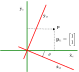
\includegraphics[width=\linewidth]{media/rot-2D.pdf}
\caption{The coordinate  frame $\{C\}$  is rotated around origin by an $\theta$
  from coordinate  frame $\{W\}$.}
\label{fig:rot-2D}
\end{figure}

\begin{thm}[Orthogonality of 2D Rotation matrices]
  All 2D rotation matrices  are orthogonal $R^\top R = I$ have determinant as one
  $\det(R) =  1$. If any square matrix $A \in \bbR^{2\times  2}$ is orthogonal $A^\top A = I$  and has
  determinant 1, $\det(A) = 1$, then  it is a valid rotation matrix.
\end{thm}
\begin{proof}
  \begin{align}
    R^\top R
    &= \begin{bmatrix}
      \cos(\theta)  &  -\sin(\theta)
      \\
      \sin(\theta) &   \cos(\theta)
    \end{bmatrix}^\top \begin{bmatrix}
      \cos(\theta)  &  -\sin(\theta)
      \\
      \sin(\theta) &   \cos(\theta)
    \end{bmatrix}
    \notag\\
    &=\begin{bmatrix}
      \cos(\theta)  &  \sin(\theta)
      \\
      -\sin(\theta) &   \cos(\theta)
    \end{bmatrix} \begin{bmatrix}
      \cos(\theta)  &  -\sin(\theta)
      \\
      \sin(\theta) &   \cos(\theta)
    \end{bmatrix}
  \notag\\
    &=\begin{bmatrix}
      \cos^2(\theta)+\sin^2(\theta)  &  -\cos(\theta)\sin(\theta)+\sin(\theta)\cos(\theta)
      \\
      -\sin(\theta)\cos(\theta)+\cos(\theta)\sin(\theta) &   \sin^2(\theta)+\cos^2(\theta)
    \end{bmatrix}
\notag\\
    &=\begin{bmatrix}
      1  &  0  \\ 0  &   1\end{bmatrix}
    \end{align}
    \begin{align}
      \det(R) &
                =  \det\begin{bmatrix}
        \cos(\theta)  &  -\sin(\theta)
        \\
        \sin(\theta) &   \cos(\theta)
        \end{bmatrix}
                       \notag\\
              &= \cos^2(\theta)+  \sin^2(\theta)  = 1
      \end{align}
  Denote the columns of square matrix $A$ which  is orthogonal with determinant
  1 as $A = [\bfa_1, \bfa_2]$. Since $A$ is orthogonal,  we have
  \begin{align}
    A^\top A
    &= \begin{bmatrix}
      \bfa_1^\top  \\   \bfa_2^\top
    \end{bmatrix}
    \begin{bmatrix}
      \bfa_1  &   \bfa_2
    \end{bmatrix}  = \begin{bmatrix} \bfa_1^\top \bfa_1  & \bfa_1^\top \bfa_2
      \\
      \bfa_2^\top \bfa_1 & \bfa_2^\top \bfa_2\end{bmatrix}
      \notag\\
    &= \begin{bmatrix} 1  &  0   \\  0  &  1 \end{bmatrix}.
  \end{align}
  This   implies that $\bfa_1$  and  $\bfa_2$ are mutually orthogonal unit
  vectors. Let $\bfa_1  = [\cos(\theta), \sin(\theta)]$ because any 2D unit
  vector can  be written in cos,sin form, where $\theta = \atantwo(a_{12}, a_{11})$.
  Next we know  that  $\bfa_1^\top\bfa_2 =  0$ and that $\bfa_2$ is unit  vector.
  For any  unit 2D vector   $[u, v]^\top$, there are only two unit vectors
  perpendicular to it $[-v, u]^\top$ and $[v, -u]^\top$.
  Then we have only two
  options for $\bfa_2$  are  either $[-\sin(\theta), \cos(\theta)]$ or
  $[\sin(\theta), -\cos(\theta)]$.  But we also  know that the determinant of
  $A$ is  1. The second option   for $\bfa_2$ leads to determinant of -1.
  \begin{align}
    \det\begin{bmatrix}
      \bfa_1  &  \bfa_2
      \end{bmatrix}
    &=  
      \det\begin{bmatrix}
        \cos(\theta)  &  \sin(\theta)\\
        \sin(\theta) &  -\cos(\theta)
      \end{bmatrix} = -1
    \end{align}
    Hence, we have
    \[
      A = \begin{bmatrix}
        \bfa_1  &  \bfa_2
      \end{bmatrix}
      =  
      \begin{bmatrix}
        \cos(\theta)  &  -\sin(\theta)\\
        \sin(\theta) &  \cos(\theta)
      \end{bmatrix} = R(\theta) \]

\end{proof}

\section{2D Transformation matrix}

To consider the rotation and  translation case, we consider  the case shown in Fig~\ref{fig:rot+trans-2D}.
We have  an  intermediate frame $\{I\}$ which has only  rotation from $\{C\}$
frame. We assume that basis   vectors  $\{I\}$ are parallel to $\{W\}$ which
make it translation only conversion. We can convert  from $\bfp_c$ to $\bfp_I$
using  the rotation   matrix  derived  in the previous section,
%
\begin{align}
  \bfp_I  &=  B_I^{-1} B_c \bfp_c = R(\theta) \bfp_c.
\end{align}
%
We can account  for the  translation of the frame $\bfp_I$ by noticing that the
coordinate frames only  differ  in  origin, such that $B_c\bfo_c =  B_w(\bfo_w +
{}^w\bft_c)$, where   the  translation ${}^w\bft_c$ is  measured in  world
coordinate  frame.
\begin{align}
  \bfp  &=   B_c (\bfp_c + \bfo_c) =   B_w (\bfp_w  +  \bfo_w)
  \notag\\
  \implies   &B_c \bfp_c + B_c \bfo_c =   B_w \bfp_w  +  B_w \bfo_w
\notag\\
  \implies   &B_c \bfp_c + (B_c \bfo_c -  B_w \bfo_w)  =   B_w \bfp_w  
\notag\\
  \implies   &B_c \bfp_c + B_w {}^w\bft_c  =   B_w \bfp_w  
\notag\\
  \implies   &B_w^{\top}  B_c \bfp_c + {}^w\bft_c  =   \bfp_w  
\notag\\
  \implies   &\bfp_w = R(\theta) \bfp_c + {}^w\bft_c
\end{align}

\newcommand{\ubfp}{\underline{\bfp}}
This relation is often written  in  terms of homogeneous   coordinates  which
are   obtained by  appending 1 to euclidean coordinates  $\ubfp_w
= \begin{bmatrix}
  \bfp_w \\ 1   \end{bmatrix}$ and  $\ubfp_c
= \begin{bmatrix}
  \bfp_c \\ 1   \end{bmatrix}$.

The matrix that transforms homogeneous coordinates in one  coordinate  frame to
another is called the transformation matrix. For  2D  systems it is  $3 \times
3$ matrix denoted  by ${}^wT_c$,
%
\begin{align}
  \ubfp_w = \begin{bmatrix}
    R(\theta) & {}^w\bft_c  \\
    \boldsymbol{0}^\top &  1
  \end{bmatrix}  \ubfp_c  = {}^wT_c \ubfp_c
\end{align}
%

\begin{figure}
  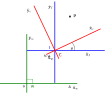
\includegraphics[width=\linewidth]{media/rot+trans-2D.pdf}
  \caption{The coordinate  frame $\{C\}$  is rotated around origin by an $\theta$
    from coordinate  frame $\{W\}$ and then shifted by translation ${}^w\bft_c$.}
  \label{fig:rot+trans-2D}
\end{figure}

\section{Principal 3D  Rotations}
\includegraphics[width=\linewidth]{media/euler-angles.pdf}
2D Rotation can be  easily extended to rotation around an axis  in 3D.  Rotation
around  X-axis, Y-axis, Z-axis   is respectively given  by,
\begin{align}
  R_x(\phi) &= \text{Roll}(\phi)  = \begin{bmatrix}
    1  &  0 &  0 \\
    0  &  \cos(\phi)  &  -  \sin(\phi) \\
    0  &  \sin(\phi)  &  \cos(\phi)
    \end{bmatrix}
  \notag\\
  R_y(\theta) & = \text{Pitch}(\theta)  = \begin{bmatrix}
    \cos(\phi)  &  0 &  \sin(\phi) \\
    0  &  1 &  0 \\
    -\sin(\phi)  &   & \cos(\phi)
  \end{bmatrix}
\notag\\
  R_z(\psi) & = \text{Yaw}(\psi)  = \begin{bmatrix}
    \cos(\psi)  &  -  \sin(\psi)  & 0    \\
    \sin(\psi)  &  \cos(\psi)  &  0   \\
    0 &  0     &   1
  \end{bmatrix}
\end{align}
\section{3D  Rotation matrix   from Euler  angles}
Euler  angles   can be applied sequentially  in  one  of the two ways:
\begin{enumerate}
  \item Proper Euler angles (z-x-z, x-y-x, y-z-y, z-y-z, x-z-x, y-x-y)
  \item Tait-Bryan angles   (x-y-z, y-z-x, z-x-y, x-z-y, z-y-x, y-x-z).
  \end{enumerate}
  
One of the most  common application  of Euler angles is X-Y-Z:
\begin{align}
  R(\phi, \theta, \psi) = R_z(\psi)R_y(\theta)R_x(\phi) = \text{Yaw}(\psi)\text{Pitch}(\theta)\text{Roll}(\phi).
\end{align}
Note that the rotation matrix  application is read  from right  to  left.

\begin{align}
  &R(\phi, \theta, \psi) =  \begin{bmatrix}
  c_\psi & - s_\psi & 0 \\
  s_\psi & c_\psi & 0 \\
  0 & 0 & 1
  \end{bmatrix}
  \begin{bmatrix}
    c_\theta & 0 & s_\theta \\
    0 & 1 & 0 \\
    - s_\theta & 0 & c_\theta
    \end{bmatrix}
    \begin{bmatrix}
      1 & 0 & 0 \\
      0 & c_\phi & - s_\phi \\
      0 & s_\phi & c_\phi
      \end{bmatrix}
\notag\\&\quad
  =\begin{bmatrix}
    c_\psi & - s_\psi & 0 \\
    s_\psi & c_\psi & 0 \\
    0 & 0 & 1
  \end{bmatrix}
            \begin{bmatrix}
              c_\theta & s_\theta s_\phi & s_\theta c_\phi \\
              0 & c_\phi & -s_\phi \\
              -s_\theta & c_\theta s_\phi & c_\theta c_\phi
            \end{bmatrix}
\notag\\&\quad
  = \begin{bmatrix}
    c_\psi c_\theta & c_\psi s_\theta s_\phi - s_\psi c_\phi & c_\psi s_\theta c_\phi+ s_\psi s_\phi \\
    s_\psi c_\theta & s_\psi s_\theta s_\phi + c_\psi c_\phi & s_\psi s_\theta c_\phi - c_\psi s_\phi \\
    -s_\theta & c_\theta s_\phi & c_\theta c_\phi
    \end{bmatrix}
\end{align}

For a  given 3D  rotation matrix $R$, whose   elements  are   $r_{ij}$ as follows
%
\begin{align}
R =  \begin{bmatrix}
  r_{11}  &   r_{12} &   r_{13}   \\
  r_{21}  &   r_{22} &   r_{23}   \\
  r_{31}  &   r_{32} &   r_{33} 
  \end{bmatrix},
\end{align}
%
the roll,  pitch, yaw  angles can  be read as,
\begin{align}
  \phi &= \atantwo(r_{32},   r_{33}) \\
  \theta &= -\arcsin(r_{31}) \\
  \psi &= \atantwo(r_{22}, r_{21})
  \end{align}

\subsection{Gimbal lock}

When pitch $\theta  = \frac{\pi}{2}$, then yaw-axis (Z-axis) coincides with
roll-axis (X-axis). In such a  case,  inversion from a rotation matrix leads to
infinitely possible solutions, because  $c_\theta = 0$ and   that leads  to
$r_{32} = r_{33} =  r_{22} = r_{21} = 0$.

\subsection{Orthogonality and determinant}
Let 3D rotation  be represented  by a block matrix of 2D rotation $R_2(\phi)$.
\[
  R_x(\phi) = \begin{bmatrix}
          1  &   \boldsymbol{0}^\top   \\
               \boldsymbol{0}  &   R_2(\phi)
          \end{bmatrix}
\]

\begin{align}
  &R_x^\top(\phi) R_x(\phi) =  \begin{bmatrix}
    1  &   \boldsymbol{0}^\top   \\
    \boldsymbol{0}  &   R_2(\phi)
  \end{bmatrix}^\top
  \begin{bmatrix}
    1  &   \boldsymbol{0}^\top   \\
    \boldsymbol{0}  &   R_2(\phi)
  \end{bmatrix}
 \notag\\
  &\quad
 =
  \begin{bmatrix}
    1  &   \boldsymbol{0}^\top   \\
    \boldsymbol{0}  &   R_2^\top(\phi)R_2(\phi)
  \end{bmatrix}
                      = I
\end{align}

Same  check can be applied to $R_y(\theta)$ and  $R_z(\psi)$  as   well. If two
matrices  $A$ and  $B$ are orthogonal, then $AB$ is also orthogonal:
\begin{align}
  (AB)^\top(AB)  = B^\top A^\top A B =   B^\top I  B =  B^\top B = I.
\end{align}

Hence any combination of principal rotations is also orthogonal.

Similar procedure can  be followed to establish  that  $\det(R) = 1$.

\section{3D  Transformation matrix}
For  3D  systems transformation matrix is  $4 \times 4$ matrix denoted  by ${}^wT_c$,
% 
\begin{align}
  \ubfp_w = \begin{bmatrix}
    R(\phi, \theta, \psi) & {}^w\bft_c  \\
    \boldsymbol{0}^\top &  1
  \end{bmatrix}  \ubfp_c  = {}^wT_c \ubfp_c,
\end{align}
% 
where  ${}^w\bft_c   \in \bbR^3$, $\ubfp_c =  \begin{bmatrix} \bfp_c   \\
  1   \end{bmatrix}$ and $\bfp_c  \in \bbR^3$.


\section{Axis-angle representation}
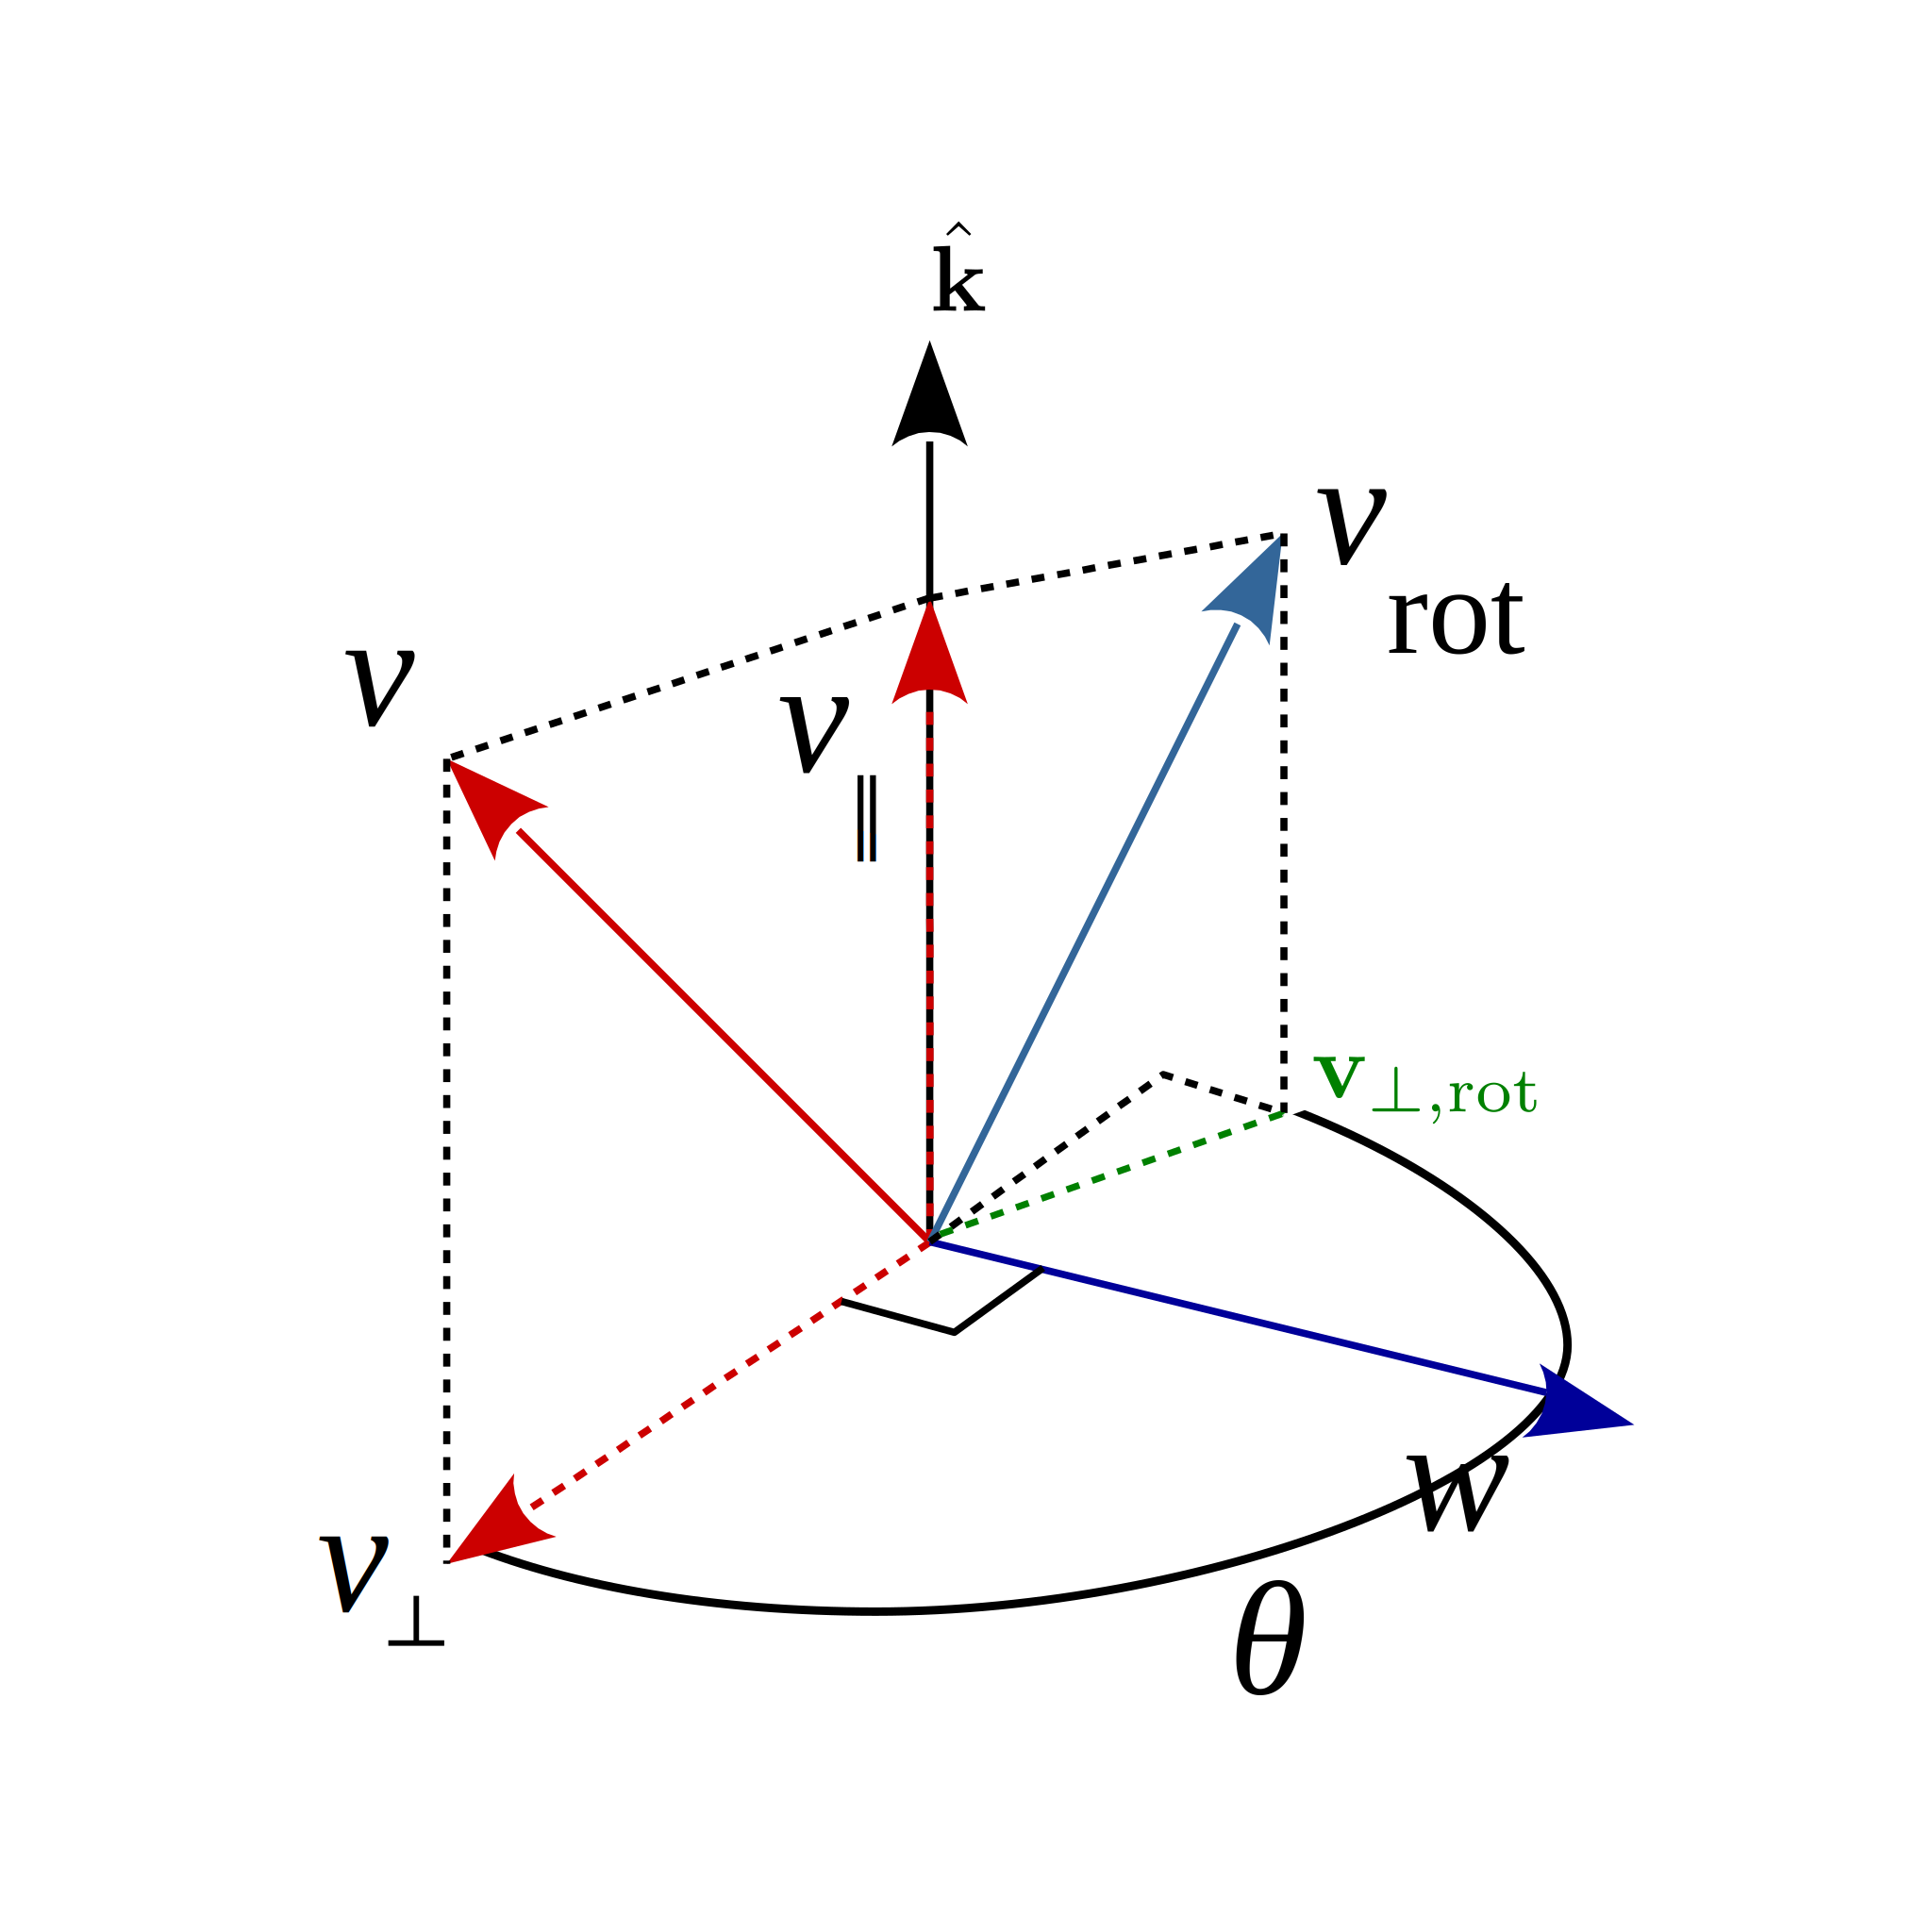
\includegraphics[width=\linewidth]{media/Rodrigues-formula.pdf}
%
Cross product gives us a vector that is orthogonal to the plane of two vectors,
let $\bfw = \hat{\bfk} \times \bfv$ be such a vector. Note that the magnitude of
$\bfw$, $\|\bfw\| = \|\hat{\bfk}\| \bfv \sin(\phi)$, where $\phi$ is the angle
between the unit-vector $\hat{\bfk}$ and $\bfv$.
\begin{align}
  \bfv_\perp &= - \hat{\bfk} \times \bfw = -  \hat{\bfk} \times (\hat{\bfk} \times \bfv)
\end{align}
\begin{align}
  \bfv_{\perp,\text{rot}}  &= \bfv_\perp\cos(\theta) + \bfw\sin(\theta)
  \\
  \bfv_{\text{rot}} &=  \bfv_\parallel +   \bfv_{\perp,\text{rot}}
  \notag\\
       &=  \bfv - \bfv_\perp +   \bfv_\perp\cos(\theta) + \bfw\sin(\theta)
  \notag\\
       &=  \bfv - (1-\cos(\theta)) \bfv_\perp + \bfw \sin(\theta)
  \notag\\
       &=  \bfv + (1-\cos(\theta)) \hat{\bfk} \times (\hat{\bfk} \times \bfv) +  \sin(\theta) \hat{\bfk} \times \bfv
\end{align}

Define  cross  product matrix $K$  of $\hat{\bfk} = \begin{bmatrix}  k_x \\ k_y
  \\ k_z \end{bmatrix}$  as,
\begin{align}
  K  = \begin{bmatrix}
    0   & - k_z & k_y   \\
    k_z   & 0 & -k_x   \\
    -k_y   & k_x & 0
  \end{bmatrix}.
\end{align}

\begin{align}
\bfv_{\text{rot}} &=  \bfv + (1-\cos(\theta)) \hat{\bfk} \times (\hat{\bfk} \times \bfv) +  \sin(\theta) \hat{\bfk} \times \bfv
                    \notag\\
  &= (I + (1 -\cos(\theta)) K^2  + \sin(\theta) K)\bfv
\end{align}

Thus the rotation matrix corresponding  to axis-angle $\theta, \hat{\bfk}$ is
given by,
%
\begin{align}
  R(\theta, \hat{\bfk}) = I + \sin(\theta)K + (1-\cos(\theta))K^2
\end{align}
%

To get back $\theta$ and $\hat{\bfk}$   from $R$,  first  note that,
% 
\begin{align}
  K^2 =  \begin{bmatrix}
    -k_z^2  - k_y^2  & k_x k_y & k_z k_x \\
    k_xk_y  & -k_x^2- k_z^2 & k_z k_y \\
    k_x k_z  & k_y k_z &  -k_x^2  - k_y^2
    \end{bmatrix} 
\end{align}
% 
Also we can use trace to separate $\theta$ from axis,
%
\begin{align}
  \tr(R) &= \tr(I)  + \sin(\theta)\tr(K) + (1-\cos(\theta))\tr(K^2)
  \notag\\
  &= 3 + 0 + (1-\cos(\theta))(-2(k_x^2 + k_y^2 + k_z^2)).
    \notag\\
  &= 3 - 2 +2\cos(\theta)
\end{align}
%
Thus we get $\theta  =  \arccos(\frac{\tr(R)-1}{2})$. We can estimate axis of
rotation as the  eigenvector corresponding  eigenvalue 1,   because $R\hat{\bfk}
= \hat{\bfk}$.

%\section{Denavit-Hartenberg  transformations}

\begin{prob}
  Degrees of Freedom of a quantity is the number independent scalar variables
  needed to represent that quantity. What is degrees of freedom required to 
  \begin{enumerate}
    \item Position and orientation in 1-D
    \item Position and orientation in 2-D
    \item Position and orientation in 3-D
    \item Position and orientation in 4-D
  \end{enumerate} (10 marks. Estimated time: 15 min)
  Justify your answer.
\end{prob}

\ifsol
\paragraph*{Solution}
\begin{enumerate}
  \item 1D: position requires 1-DoF,  orientation requires a binary flag.
  \item 2D: position requires 2-DoF, orientation requires a single angle: 1-DoF.
  \item 3D: position requires 3-DoF, orientation requires 3-DoF because there
    are three pairs of axis X-Y, Y-Z, Z-X.
  \item 4D: position requires 4-DoF, orientation requires 6-DoF because there
    are 6 pairs of axis: $^4C_2 = 6$.
\end{enumerate}
\fi

\begin{prob}
  Write a program in C++ that checks if a given
  3x3 matrix is a valid Rotation matrix is a valid Rotation matrix  (check for
  orthonormality i.e. orthogonality and determinant = 1). You may use Eigen's
  matrix multiplication and determinant() function. (10 marks. Used in the
  following problems. Estimated time: 15 min). 
\end{prob}

\ifsol
\paragraph*{Solution}
Please look at the function \verb|is_valid_rot| in file \verb|hw1.cpp|.
\fi

\begin{prob}
  In class, we proved the expression to convert roll ($\theta$), pitch
  ($\phi$), yaw ($\psi$) from Euler Angles to Rotation matrix,
  \begin{align}
    R(\theta, \phi, \psi) =
    \begin{bmatrix}
      r_{11}& r_{12} & r_{13} \\
      r_{21}& r_{22} & r_{23} \\
      r_{31}& r_{32} & r_{33}
    \end{bmatrix} 
                       = R_z(\psi) R_y(\phi) R_x(\theta).
  \end{align}
  
  What if we want to do the inverse? Prove that given a proper 3x3 rotation
  matrix  ($R^\top R = I$ and $det(R) = 1$) , the Euler angles are given by
  \begin{align}
    \begin{bmatrix}
    \theta(R) \\
    \phi(R) \\
    \psi(R)
    \end{bmatrix}
    = \begin{bmatrix}
      \atantwo(r_{32}, r_{33}) \\
      -\arcsin(r_{31}) \\
      \atantwo(r_{21}, r_{11})
      \end{bmatrix}
  \end{align}
  where $r_{ij}$ is the element in $i$th row and $j$th column of the rotation
  matrix $R$. (10 marks. Used in the
  following problems. Estimated time: 15 min).
\end{prob}

\ifsol
\paragraph*{Solution}
\begin{align}
&R(\theta, \phi, \psi) = \begin{bmatrix}
  c_\psi & - s_\psi & 0 \\
  s_\psi & c_\psi & 0 \\
  0 & 0 & 1
  \end{bmatrix}
  \begin{bmatrix}
    c_\phi & 0 & s_\phi \\
    0 & 1 & 0 \\
    - s_\phi & 0 & c_\phi
    \end{bmatrix}
 \notag\\&\quad
    \begin{bmatrix}
      1 & 0 & 0 \\
      0 & c_\theta & - s_\theta \\
      0 & s_\theta & c_\theta
      \end{bmatrix}
\notag\\&\quad
  =\begin{bmatrix}
    c_\psi & - s_\psi & 0 \\
    s_\psi & c_\psi & 0 \\
    0 & 0 & 1
  \end{bmatrix}
            \begin{bmatrix}
              c_\phi & s_\phi s_\theta & s_\phi c_\theta \\
              0 & c_\theta & -s_\theta \\
              -s_\phi & c_\phi s_\theta & c_\phi c_\theta
            \end{bmatrix}
\notag\\&\quad
  = \begin{bmatrix}
    c_\psi c_\phi & c_\psi s_\phi s_\theta - s_\psi c_\theta & c_\psi s_\phi c_\theta+ s_\psi s_\theta \\
    s_\psi c_\phi & s_\psi s_\phi s_\theta + c_\psi c_\theta & s_\psi s_\phi c_\theta - c_\psi s_\theta \\
    -s_\phi & c_\phi s_\theta & c_\phi c_\theta
    \end{bmatrix}
\end{align}

Starting from the first term of R.H.S. of the equation to be proved,
%
\begin{mutline}
  \atantwo(r_{32}, r_{33})
  = \atantwo(c_\phi s_\theta, c_\phi c_\theta) = \tan^{-1}(\frac{c_\phi
    s_\theta}{c_\phi c_\theta}) = \tan^{-1}(\frac{s_\theta}{c_\theta}) =
  \tan^{-1}(\tan(\theta)) = \theta.
\end{mutline}
%
For the second term, $-\arcsin(r_{31}) = -\sin^{-1}(-s_\phi) =  \phi$.
For the third term ,
\begin{mutline}
  \atantwo(r_{21}, r_{11})
  = \atantwo(s_\psi c_\phi, c_\psi c_\phi) = \tan^{-1}(\frac{s_\psi
    c_\phi}{c_\psi c_\phi}) = \tan^{-1}(\frac{s_\psi}{c_\psi}) =
  \tan^{-1}(\tan(\psi)) = \psi.
\end{mutline}

\fi

\begin{prob}
  Write a pair of functions in C++ that converts rotation matrix from XYZ Euler
angles (roll, pitch, yaw) and vice versa. Test the pair of functions with
randomly generated Euler angles. And check if the converted rotation matrix is
orthonormal. What happens when pitch = $\pi/2$, are you able to convert from
rotation matrix to Euler angle? Why or why not? (50 marks. Estimated time: 30 min)
\label{prob:euler-to-rotmat}
\end{prob}

\ifsol
\paragraph*{Solution}
Please check function \verb|euler_to_rotmat| and \verb|rotmat_to_euler_rpy| in
\verb|hw1.cpp|. When pitch $=\frac{\pi}{2}$ works some of the time, but not all the time because of the
Gimbal lock matrix to Euler angle conversion has multiple possible solutions.
\fi

\begin{prob}
  Write a function in C++ that generates a 4x4 transformation matrix given XYZ Euler
  angles (roll, pitch, yaw) and translation. You can use the function that you
  wrote in Prob~\ref{prob:euler-to-rotmat}(20 marks. Estimated time: 15 min).
\end{prob}

\ifsol
\paragraph*{Solution}
Please check function \verb|transformation_matrix| in \verb|hw1.cpp|
\fi


\begin{prob}
  In class we proved the Rodrigues formula that converts from axis-angle
  representation $(\theta, \hat{\bfk})$, where $\theta$ is the angle of rotation
  and $\hat{\bfk}$ is the axis of rotation ($\|\hat{\bfk}\| = 1$). Let $\bfK = [\hat{\bfk}]_{\times}$ be
  the cross product matrix of $\hat{\bfk}$. The cross product matrix
  of $\hat{\bfk} = [k_x, k_y, k_z]^\top$ (such that $k_x^2 + k_y^2 + k_z^2 = 1$) is defined as,
    \begin{align}
      \bfK = [\hat{\bfk}]_{\times} = \begin{bmatrix}
        0 & -k_z & k_y \\
        k_z & 0 & -k_x \\
        -k_y & k_x & 0
      \end{bmatrix}
    \end{align}
  The corresponding rotation matrix is
  given by,
  \begin{align}
    R(\theta, \hat{\bfk}) = \bfI + \sin \theta \bfK + (1-cos \theta) \bfK^2.
  \end{align}

  An exponential of a square matrix $\bfM$ is defined as
  \begin{align}
    \exp(\bfM) = \sum_{n=0}^\infty \frac{1}{n!} \bfM^k = \bfI + \frac{1}{1!}\bfM + \frac{1}{2!}\bfM^2 + \dots
  \end{align}

  Recall the series expansion of $\sin \theta$, and $\cos \theta$,
  \begin{align}
    \sin \theta = \theta - \frac{\theta^3}{3!} + \frac{\theta^5}{5!} - \dots
    \\
    \cos \theta = 1 - \frac{\theta^2}{2!} + \frac{\theta^4}{4!} - \dots
  \end{align}

  \begin{enumerate}
  \item First prove that $\bfK^3 = - \bfK$. (15 marks, 15 minutes)
  \item As a result note that $\bfK^4 = - \bfK^2$, $\bfK^5 = \bfK$, and so on.
    In general, $\bfK^{2n+1} =
    (-1)^n\bfK$ and $\bfK^{2n+2} = (-1)^n\bfK^2$. Using the expansion of $\sin\theta$ and $\cos\theta$, prove that
    $R(\theta, \hat{\bfk}) = \exp(\theta \bfK)$. (30 marks, 30 minutes)
  \end{enumerate}
\end{prob}
\ifsol
\paragraph*{Solution}
Expanding $\bfK^2$
\begin{align}
  \bfK^2 &= \begin{bmatrix}
    0 & -k_z & k_y \\
    k_z & 0 & -k_x \\
    -k_y & k_x & 0
  \end{bmatrix}
                 \begin{bmatrix}
                   0 & -k_z & k_y \\
                   k_z & 0 & -k_x \\
                   -k_y & k_x & 0
                 \end{bmatrix}
  \\
         &= \begin{bmatrix}
           -k_z^2 - k_y^2  & k_y k_x & k_z k_x \\
           k_xk_y & -k_z^2 - k_x^2 & k_z k_y \\
           k_x k_z & k_y k_z & -k_y^2 - k_x^2
         \end{bmatrix}.
\end{align}
Expanding $\bfK^3$,
\begin{align}
  &\bfK^3 = \begin{bmatrix}
    0 & -k_z & k_y \\
    k_z & 0 & -k_x \\
    -k_y & k_x & 0
  \end{bmatrix}
                 \notag\\&\qquad
         \begin{bmatrix}
           -k_z^2 - k_y^2  & k_y k_x & k_z k_x \\
           k_xk_y & -k_z^2 - k_x^2 & k_z k_y \\
           k_x k_z & k_y k_z & -k_y^2 - k_x^2
         \end{bmatrix}
  \\&=
  \begin{bmatrix}
    -k_xk_yk_z +k_xk_yk_z & k_z (k_z^2 + k_x^2 + k_y^2) & -k_y (k_z^2 + k_x^2 + k_y^2)\\
    -k_z (k_z^2 + k_x^2 + k_y^2) & -k_xk_yk_z +k_xk_yk_z & k_x (k_z^2 + k_x^2 + k_y^2)\\
    k_y (k_z^2 + k_x^2 + k_y^2) & -k_x (k_z^2 + k_x^2 + k_y^2) & -k_xk_yk_z +k_xk_yk_z
    \end{bmatrix}
\end{align}
We know that $k_x^2 + k_y^2 + k_z^2 = 1$. Applying that we get the desired
result, $\bfK^3 = - \bfK$.

Expanding Rodrigues formula using expansion of $\sin\theta$ and $\cos\theta$, we
get
\begin{align}
  R(\theta, \hat{\bfk}) = \bfI + \bfK(\theta - \frac{\theta^3}{3!} + \frac{\theta^5}{5!}  - \dots) + \bfK^2(\frac{\theta^2 }{2!} - \frac{\theta^4}{4!} + \dots )
\end{align}
Now, note that $\bfK^3 = -\bfK$, $\bfK^4 = -\bfK^2$, $\bfK^5 = \bfK$. Moving
$\bfK$ inside the series with $\theta$, we get
\begin{align}
  &R(\theta, \hat{\bfk}) = \bfI + (\theta\bfK + \frac{(\theta\bfK)^3}{3!} + \frac{(\theta\bfK)^5}{5!}  + \dots)
    \notag\\
  &\quad
  + (\frac{(\theta\bfK)^2 }{2!} + \frac{(\theta\bfK)^4}{4!} + \dots )
  \end{align}
  This is exactly the series expansion of $\exp(\theta\bfK)$ by definition.
\fi

\begin{prob}
  Write a pair of functions in C++ that converts rotation matrix from axis-angle
  representation and vice versa. Recall that
  \begin{align}
    R(\theta, \hat{\bfk}) = \bfI + \sin \theta \bfK + (1-cos \theta) \bfK^2.
  \end{align}
  and to get axis-angle back from a given rotation matrix
  \begin{align}
    R = \begin{bmatrix}
      r_{11} & r_{12} & r_{13} \\
      r_{21} & r_{22} & r_{23} \\
      r_{31} & r_{32} & r_{33}
      \end{bmatrix},
  \end{align}
  we have
  \begin{align}
    \theta &= \cos^{-1} \left(\frac{\text{tr}(R) - 1}{2}\right)
    \\
    \hat{\bfk} &= \frac{1}{2\sin\theta}\begin{bmatrix}
      r_{32} - r_{23} \\
      r_{13} - r_{31} \\
      r_{21} - r_{12}
      \end{bmatrix} \text{ if  } \theta \ne 0 \text{ or } \pi.
  \end{align}
 If $\theta = 0 \text{ or } \pi$, then
 \begin{align}
   \hat{\bfk} = \pm\begin{bmatrix}
    \sqrt{(r_{11} + 1)/2}\\
    \sqrt{(r_{22} + 1)/2}\\
    \sqrt{(r_{33} + 1)/2}
   \end{bmatrix}
   \end{align}
  
  (30 marks. Estimated time: 30 min)
  \label{prob:euler-to-rotmat}
\end{prob}


\begin{prob}
  Recall the definition of Denavit-Hartenberg parameters from the
  \href{https://www.youtube.com/watch?v=rA9tm0gTln8}{video}. Recall that
  transformation between two joints for the defined parameters $d, \theta, r,
  \alpha$ is given by,
  \begin{align}
    T = T_z(\theta, d) T_x(\alpha, r),
  \end{align}
  where
  \begin{align}
    T_x(\alpha, r) &= \begin{bmatrix}
      1 & 0 & 0 & r \\
      0 & \cos(\alpha) & -\sin(\alpha) & 0 \\
      0 & \sin(\alpha) & \cos(\alpha) & 0 \\
      0 & 0 & 0 & 1 \\
      \end{bmatrix}
    \\
    T_z(\theta, d) &= \begin{bmatrix}
      \cos(\theta) & -\sin(\theta) & 0 &  0 \\
      \sin(\theta) & \cos(\theta) & 0  & 0 \\
      0 & 0 & 1 & d & \\
      0 & 0 & 0 & 1 &
    \end{bmatrix}
  \end{align}

  For the robot given below find transformation matrix from joint 4 to joint 1
  assuming the joint angles to be  $\theta_1$, $\theta_2$, $\theta_3$
  respectively. Write the expression for ${}^3T_4(\theta_3)$, ${}^2T_3(\theta_2)$, ${}^1T_2(\theta_1)$
  and then ${}^1T_4(\theta_1, \theta_2, \theta_3)$ in terms of the first three
  transformations. You do not need to expand the expression of  ${}^1T_4(\theta_1, \theta_2, \theta_3)$.
  \\
  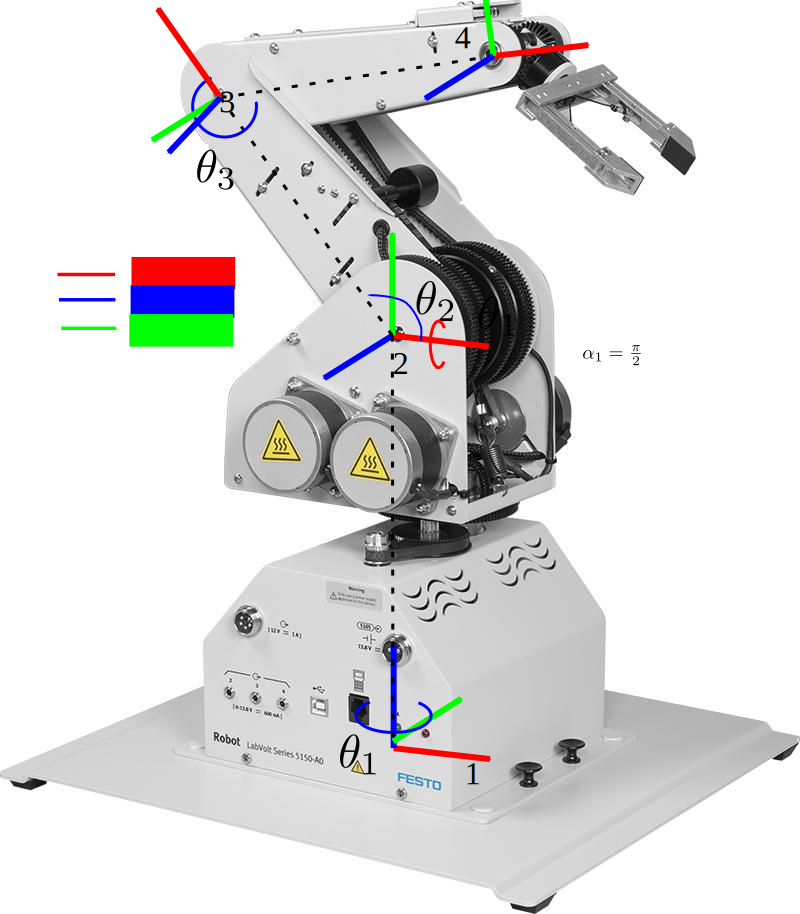
\includegraphics[width=\linewidth]{media/robot3D.pdf}
  \\
  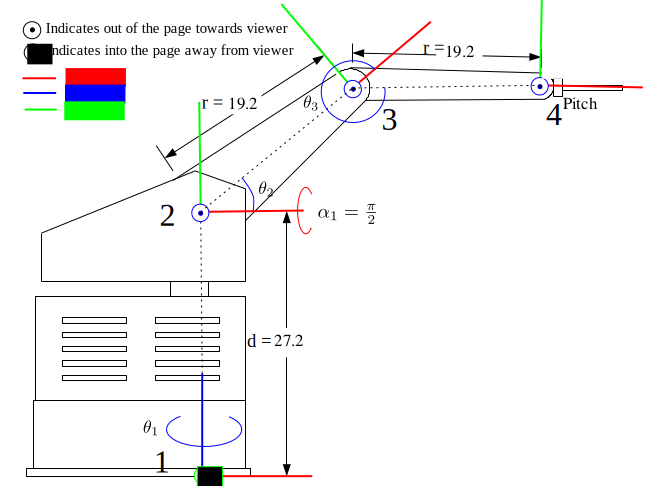
\includegraphics[width=\linewidth]{media/robot.pdf}
  (15 marks. 15 min)
\end{prob}
\ifsol
\paragraph*{Solution}
\begin{align}
  &{}^3T_4(\theta_3) =
                      \begin{bmatrix}
                        cos(\theta_3) & -\sin(\theta_3) & 0 & 0 \\
                        sin(\theta_3) & cos(\theta_3) & 0 & 0 \\
                        0 & 0 & 1 & 0 \\
                        0 & 0 & 0 & 1
                      \end{bmatrix}
                      \begin{bmatrix}
    1 & 0 & 0 & 19.2 \\
    0 & 1 & 0 & 0 \\
    0 & 0 & 1 & 0 \\
    0 & 0 & 0 & 1
  \end{bmatrix}
                \notag\\
  &\quad= \begin{bmatrix}
    cos(\theta_3) & -\sin(\theta_3) & 0 & 19.2\cos(\theta_3) \\
    sin(\theta_3) & cos(\theta_3) & 0 & 19.2\sin(\theta_3) \\
    0 & 0 & 1 & 0 \\
    0 & 0 & 0 & 1
  \end{bmatrix}
\end{align}

\begin{align}
  &{}^2T_3(\theta_2) =
    \begin{bmatrix}
      cos(\theta_2) & -\sin(\theta_2) & 0 & 0 \\
      sin(\theta_2) & cos(\theta_2) & 0 & 0 \\
      0 & 0 & 1 & 0 \\
      0 & 0 & 0 & 1
    \end{bmatrix}
                  \begin{bmatrix}
                    1 & 0 & 0 & 19.2 \\
                    0 & 1 & 0 & 0 \\
                    0 & 0 & 1 & 0 \\
                    0 & 0 & 0 & 1
                  \end{bmatrix}
                                \notag\\
  &\quad= \begin{bmatrix}
    cos(\theta_2) & -\sin(\theta_2) & 0 & 19.2\cos(\theta_2) \\
    sin(\theta_2) & cos(\theta_2) & 0 & 19.2\sin(\theta_2) \\
    0 & 0 & 1 & 0 \\
    0 & 0 & 0 & 1
  \end{bmatrix}
\end{align}

\begin{align}
  &{}^1T_2(\theta_1) =
    \begin{bmatrix}
      cos(\theta_1) & -\sin(\theta_1) & 0 & 0 \\
      sin(\theta_1) & cos(\theta_1) & 0 & 0 \\
      0 & 0 & 1 & 27.2 \\
      0 & 0 & 0 & 1
    \end{bmatrix}
                  \begin{bmatrix}
                    1 & 0 & 0 & 0 \\
                    0 & 0 & -1 & 0 \\
                    0 & 1 & 0 & 0 \\
                    0 & 0 & 0 & 1
                  \end{bmatrix}
                                \notag\\
  &\quad= \begin{bmatrix}
    cos(\theta_1) & 0 & sin(\theta_1) & 0 \\
    sin(\theta_1) & 0 & -cos(\theta_1) & 0 \\
    0 & 1 & 0 & 27.2 \\
    0 & 0 & 0 & 1
  \end{bmatrix}
\end{align}
\begin{align}
  {}^1T_4(\theta_1, \theta_2, \theta_3) = {}^1T_2(\theta_1) {}^2T_3(\theta_2) {}^3T_4(\theta_3)
\end{align}
\fi
\section{Camera  projection model}

\includegraphics[width=\linewidth]{media/pinhole-camera-model-2.png}
\newcommand{\ubfu}{\underline{\bfu}}
\newcommand{\ubfX}{\underline{\bfX}}
\begin{align}
  \bfK &= \begin{bmatrix}
    f_x & s & u_0 \\
    0 & f_y & v_0 \\
    0 & 0 & 1 \\
  \end{bmatrix}
  \\
  \bfu &= \begin{bmatrix} u   \\ v \end{bmatrix} \text{ image coordinates in pixels} \\
  \bfX &= \begin{bmatrix} X   \\  Y   \\ Z\end{bmatrix} \text{ 3D coordinates in world units}\\
  \ubfu &= \begin{bmatrix} \bfu \\   1\end{bmatrix} \\
  \lambda \ubfu &= K \bfX, \text{ where } \lambda \ne 0
\end{align}
\section{Linear least squares  or  Pseudo-inverse}

Pseudo-inverse of a matrix  $\bfA$ is defined   as a matrix $\bfA^\dagger$, such
that$\bfA \bfA^\dagger \bfA =  \bfA$.
\begin{align}
  \text{if } \bfA \text{ is tall and full-col rank, then } \bfA^\dagger &= (\bfA^\top \bfA)^{-1} \bfA^\top \\
  \text{if } \bfA \text{ is fat and full-row rank, then } \bfA^\dagger &=  \bfA^\top (\bfA \bfA^\top)^{-1}
\end{align}\footnote{See Appendix A of Gilbert Strang (1988): Linear Algebra
  and Its Applications}

\begin{align}
  \min_{\bfx} &\|A\bfx - \bfb\|^2
  \\
              &= \min_\bfx (A\bfx - \bfb)^\top (A\bfx - \bfb)
  \\
              &= \min_\bfx (\bfx^\top A^\top - \bfb^\top) (A\bfx - \bfb)
  \\
              &= \min_\bfx (\bfx^\top A^\top - \bfb^\top) (A\bfx - \bfb)
  \\
              &= \min_\bfx \bfx^\top A^\top A\bfx - \bfb^\top A\bfx - \bfx^\top A^\top \bfb + \bfb^\top \bfb
\end{align}

Recall that a minimum (or maximum) point of a differentiable function $f(\bfx)$,
$f'(\bfx)  = 0$. Let us define vector derivative as

\begin{align}
  \frac{\partial f(\bfx)}{\partial \bfx} = \begin{bmatrix}
    \frac{\partial f(\bfx)}{\partial x_1}
    \\
    \frac{\partial f(\bfx)}{\partial x_2}
    \\
    \vdots
    \\
    \frac{\partial f(\bfx)}{\partial x_n}
  \end{bmatrix}
\end{align}
You can verfiy that
\begin{align}
  \frac{\partial }{\partial \bfx} \bfx^\top Q \bfx &= 2 Q\bfx
  \\
  \frac{\partial }{\partial \bfx} \bfb^\top \bfx &= \bfb
\end{align}

At a minimum point $\bfx$,
%
\begin{align}
  &\frac{\partial }{\partial \bfx} \left(\bfx^\top A^\top A\bfx - \bfb^\top A\bfx - \bfx^\top A^\top \bfb + \bfb^\top \bfb\right) = 0
\end{align}
%
Note that  $\bfb^\top A\bfx$ is a scalar, and hence $\bfb^\top A\bfx =
(\bfb^\top A\bfx)^\top = \bfx^\top A^\top \bfb$.
%
\begin{align}
  \implies & 2A^\top A\bfx - 2 A^\top \bfb = 0
  \\
  \implies & \bfx = \underbrace{(A^\top A)^{-1} A^\top}_{A^\dagger} \bfb
\end{align}

\listoftheorems[ignoreall,show={defn}]

\end{document}